% Chapter 1

\chapter{Introducción general} % Main chapter title

\label{Chapter1} % For referencing the chapter elsewhere, use \ref{Chapter1} 
\label{IntroGeneral}

%----------------------------------------------------------------------------------------

% Define some commands to keep the formatting separated from the content 
\newcommand{\keyword}[1]{\textbf{#1}}
\newcommand{\tabhead}[1]{\textbf{#1}}
\newcommand{\code}[1]{\texttt{#1}}
\newcommand{\file}[1]{\texttt{\bfseries#1}}
\newcommand{\option}[1]{\texttt{\itshape#1}}
\newcommand{\grados}{$^{\circ}$}

%----------------------------------------------------------------------------------------

%\section{Introducción}

%----------------------------------------------------------------------------------------

El Salar de Llullaillaco, ubicado en la región altoandina de la Puna argentina, constituye un ecosistema frágil y poco estudiado desde el punto de vista hidrológico. En el contexto actual de cambio climático y expansión de la minería de litio, comprender su dinámica hídrica se vuelve estratégico tanto para la conservación ambiental como para la planificación territorial. Este capítulo presenta el marco general del estudio, se aborda el contexto físico e hidroclimático de la región, el desarrollo minero en los salares, la motivación del trabajo y su encuadre dentro del estado del arte. Además, se detallan los objetivos que guían la investigación y los límites metodológicos adoptados.


\section{Contexto hídrico de la región}


La región de la Puna argentina constituye uno de los ambientes más extremos, áridos y elevados del continente sudamericano. Ubicada al noroeste del país, abarca territorios de las provincias de Jujuy, Salta y Catamarca, y se extiende a lo largo de la zona de transición entre los Andes Centrales y el Altiplano. Con altitudes que superan los 3500 metros sobre el nivel del mar, esta región se caracteriza por condiciones climáticas rigurosas: precipitaciones escasas (inferiores a 200 mm anuales), alta radiación solar, fuertes vientos y una marcada amplitud térmica diaria. En la imagen ~\ref{fig:fisiografia} se puede observar la fisiografia de la Puna argentina en un contexto de los Andes Centrales. 

Dentro de este entorno se desarrollan ecosistemas frágiles y altamente especializados, entre los que destacan los salares altoandinos, lagunas salinas y vegas. Estos cuerpos de agua, que ocupan depresiones endorreicas, tienen un comportamiento hidrológico complejo y variable, dependen fundamentalmente de la recarga superficial estacional, la infiltración y la evaporación, que es intensa durante gran parte del año. La limitada disponibilidad hídrica en la región determina no solo el desarrollo de comunidades biológicas adaptadas a condiciones extremas, sino también la viabilidad de actividades productivas como la ganadería trashumante, el turismo y, más recientemente, la minería del litio.


\begin{figure}[htpb]
	\centering
	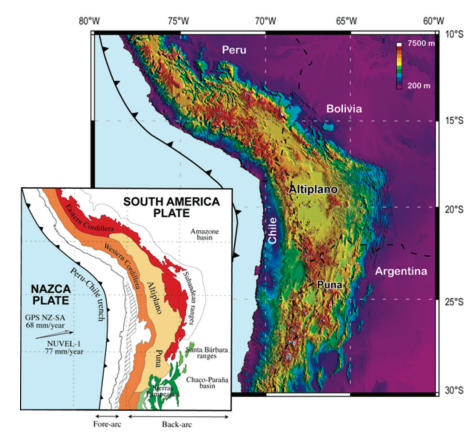
\includegraphics[scale=.6]{./Figures/fig1.png}
	\caption{Fisiografía y unidades geológicas y morfotectónicas de los Andes Centrales\protect\footnotemark.}
	\label{fig:fisiografia}
\end{figure}
\FloatBarrier

La dinámica de los sistemas acuáticos en la Puna argentina está fuertemente influenciada por las fluctuaciones interanuales en las precipitaciones y por eventos climáticos de escala global como El Niño-Oscilación del Sur (ENSO) \cite{trenberth1997definition}. Durante fases cálidas de ENSO, pueden producirse anomalías positivas de precipitación que incrementan temporalmente la superficie cubierta por agua en lagunas y salares. Sin embargo, la magnitud y frecuencia de estos eventos son irregulares y dependen de múltiples factores atmosféricos.

Uno de los principales desafíos para caracterizar estos ambientes radica en la escasez de datos \textit{in situ}. La lejanía geográfica, la falta de infraestructura de monitoreo y las condiciones climáticas adversas dificultan la observación directa y sistemática. La teledetección se usa como una herramienta clave para el estudio de la dinámica hídrica regional, como lo demuestran estudios recientes en regiones altoandinas \cite{saavedra2018changes}.

\footnotetext{Imagen tomada de  \url{https://www.researchgate.net/
publication/342886312}}


El uso de imágenes satelitales multiespectrales y técnicas de teledetección ha cobrado especial relevancia para generar series temporales extensas con datos históricos de sensores como  Landsat \cite{wulder2019landsat}. Esto permite evaluar la evolución de estos cuerpos de agua a lo largo de varias décadas, capturar patrones estacionales, eventos extremos y tendencias de largo plazo. El uso de estas herramientas y técnicas ayuda a mejorar el conocimiento ecológico de los salares y a generar insumos para la toma de decisiones en un contexto de creciente presión sobre los recursos hídricos del altiplano argentino.

%----------------------------------------------------------------------------------------

\section{Contexto del litio en la región}
La región de la Puna argentina se ha convertido en un nodo estratégico dentro del denominado Triángulo del Litio, una zona compartida con Bolivia y Chile que alberga algunas de las mayores reservas de litio del planeta. En esta área, los salares constituyen sistemas hidrogeológicos endorreicos en los que se acumulan salmueras ricas en litio, potasio, boro y otros elementos. Esta riqueza mineral ha dado lugar al despliegue de numerosos proyectos de exploración y explotación minera, particularmente enfocados en el litio en salmuera, una forma no convencional de yacimiento en la que el recurso se encuentra en estado disuelto dentro de acuíferos subterráneos.

Según un relevamiento reciente realizado por López Steinmetz et al. \cite{lopezsteinmetz2024book}, en 2023 existían al menos 90 proyectos de litio tipo salmuera anunciados en el noroeste argentino. Estos proyectos abarcan un amplio espectro de etapas, desde la prospección inicial hasta la operación productiva. Sin embargo, solo el 5,52 \% de la superficie minera otorgada está efectivamente en etapa de producción de litio. A esto se suma un dato llamativo: el 73 \% de las minas concedidas se encuentran fuera de los salares, y el 58\% de los proyectos carecen de datos sobre la concentración de litio en las salmueras, lo que introduce incertidumbres tanto técnicas como ambientales en la gestión de estos recursos.

El sector está dominado por actores privados, quienes controlan el 89\% del total de los 28 752 km² otorgados como concesiones mineras en la región andina argentina. Aun así, la industria mantiene una dinámica competitiva sin alcanzar una completa monopolización: solo tres empresas concentran el 21\% de las concesiones. Esta configuración plantea importantes desafíos para la gobernanza de los recursos, la distribución de beneficios y la gestión ambiental estratégica de los salares.

La regulación y fiscalización de los recursos hídricos en estas zonas cobra entonces una importancia crítica, dado que el proceso extractivo implica la utilización intensiva de agua subterránea, tanto en forma de salmuera como de agua dulce. Si bien representa un porcentaje reducido del uso industrial global, su impacto es significativo en contextos áridos, donde el recurso hídrico es limitado y cumple un rol fundamental para comunidades locales, fauna y ecosistemas.

En este contexto, comprender la distribución espacio-temporal del agua en los salares y su relación con los procesos climáticos se vuelve esencial no solo desde una perspectiva científica, sino también para informar políticas públicas más sostenibles y equitativas.


%----------------------------------------------------------------------------------------

\section{Motivación}

La actividad minera en los salares altoandinos requiere una gran cantidad de agua, utilizada en el bombeo de salmuera y en las operaciones auxiliares de procesamiento. Estudios recientes estiman que la huella hídrica total de un proyecto como Olaroz asciende a 584,1 m\textsuperscript{3} por tonelada de carbonato de litio, con un 92\% correspondiente a salmuera y un 8\% a agua dulce \cite{lopezsteinmetz2024book}.

En paralelo, investigaciones realizadas en el Salar de Atacama y otros sistemas similares muestran que el cambio climático reduce la cobertura nival, eleva la línea de isonieve y disminuye la persistencia estacional de los cuerpos de agua \cite{saavedra2018changes}. Estas transformaciones afectan la recarga natural de los acuíferos y agravan la presión sobre los recursos hídricos superficiales y subterráneos.

Asimismo, estudios limnológicos en lagos salinos del norte de Chile indican que las fluctuaciones térmicas estacionales y la turbidez del agua pueden ser evaluadas mediante sensores remotos como Landsat 8 \cite{delosrios2024lakes}, lo que refuerza la potencialidad de la teledetección para el monitoreo ambiental de salares en zonas remotas.

Frente a este panorama, se plantea la necesidad de contar con herramientas técnicas y replicables que permitan identificar patrones hídricos, anticipar escenarios y orientar decisiones de gestión. La combinación de datos satelitales históricos y técnicas de inteligencia artificial constituye una oportunidad concreta para modelar la ocurrencia de agua en salares y comprender su relación con variables climáticas globales como ENSO.

%----------------------------------------------------------------------------------------

\section{Estado del arte}

En los últimos años, el monitoreo ambiental de ecosistemas altoandinos mediante imágenes satelitales ha ganado relevancia en la comunidad científica. Esto se debe tanto al crecimiento de la minería de litio como a la necesidad de comprender los impactos del cambio climático sobre la disponibilidad de agua en regiones áridas. En este contexto, la combinación de datos de sensores remotos con modelos de aprendizaje automático se presenta como una herramienta robusta para detectar cambios, inferir patrones y generar predicciones sobre sistemas complejos.

Uno de los enfoques más utilizados es el procesamiento multitemporal de imágenes Landsat, que permite evaluar la presencia de cuerpos de agua a partir de índices espectrales como NDWI \textit{(Normalized Difference Water Index)}, NDVI \textit{(Normalized Difference Vegetation Index)} y NDSI \textit{(Normalized Difference Snow Index)}. Estas metodologías han sido aplicadas con éxito en estudios sobre cobertura nival en los Andes \cite{saavedra2018changes} y en la caracterización de lagos salinos mediante parámetros ópticos como turbidez o temperatura superficial \cite{delosrios2024lakes}.

En el ámbito de la minería de litio, el trabajo de López Steinmetz et al. \cite{lopezsteinmetz2024book} destaca la escasa disponibilidad de datos ambientales verificables, especialmente en lo que respecta a la disponibilidad hídrica en salares. Este vacío de información representa una oportunidad para la aplicación de modelos independientes basados en imágenes satelitales.

Por otro lado, existen antecedentes locales relevantes desarrollados en el marco de la Especialización en Inteligencia Artificial de FIUBA. Por ejemplo, Roldán \cite{roldan2023ceia} diseñó un \textit{pipeline} de procesamiento de imágenes aéreas de alta resolución para la clasificación de morfologías de cultivos mediante índices espectrales y redes neuronales convolucionales, en combinación con algoritmos de detección de líneas como la transformada de Hough. Su enfoque sobre datos geoespaciales y procesamiento espectral es comparable con el uso de Landsat en estudios ambientales, aunque aplicado al ámbito agrícola.

Asimismo, Ferrán \cite{ferran2024ceia} integró imágenes Sentinel-2 con datos de sensores terrestres para evaluar la correspondencia entre índices espectrales y observaciones en campo. Su metodología basada en Python y herramientas de código abierto como GeoPandas, Rasterio y OpenEO, puede servir de referencia para la estructuración de \textit{pipelines} multifuente orientados a monitoreo de ecosistemas.

De forma complementaria, Tentor \cite{tentor2023ceiot} desarrolló una plataforma web para la integración y visualización de datos de humedad de suelo, donde se combinan sensores IoT con imágenes satelitales y técnicas de fusión de datos. Su enfoque orientado a toma de decisiones en el ámbito agronómico puede ser extrapolado a problemáticas ambientales como la gestión de recursos hídricos en zonas de extracción minera.

En conjunto, estos antecedentes muestran que existe una base metodológica consolidada para integrar imágenes satelitales, análisis multitemporal e inteligencia artificial en estudios de carácter ambiental y productivo. Sin embargo, aún son escasos los trabajos aplicados específicamente a los salares altoandinos del noroeste argentino, lo que refuerza la pertinencia y originalidad del presente estudio.


%----------------------------------------------------------------------------------------

\section{Objetivos y alcance}

Analizar los patrones temporales de ocurrencia de agua superficial en el Salar de Llullaillaco a partir de imágenes Landsat, e investigar su relación con variables climáticas globales asociadas al fenómeno ENSO mediante técnicas de teledetección, análisis de series temporales.

Dentro de los objetivos específicos, se pueden mencionar los siguientes:

\begin{itemize}
    \item Generar series temporales de índices espectrales (NDWI) a partir de imágenes Landsat 5, 7 y 8 para identificar zonas con presencia estacional o persistente de agua superficial.
    \item Preprocesar y normalizar variables climáticas relevantes (Niño 3.4, SOI, MEI) para su análisis conjunto con los datos satelitales.
    \item Integrar y correlacionar los índices espectrales con series mensuales de indicadores climáticos globales (Niño 3.4, SOI, MEI) para evaluar relaciones potenciales.
    \item Aplicar modelos de análisis de series temporales (SARIMA y VAR) y pruebas de causalidad de Granger para identificar dependencias y relaciones dinámicas entre las variables.
    \item Entrenar y evaluar modelos de aprendizaje automático para generar predicciones exploratorias sobre la ocurrencia de agua superficial.
    \item Visualizar y analizar temporalmente los resultados mediante gráficos interpretativos y funciones de respuesta al impulso (IRF).
\end{itemize}

El alcance del trabajo se enfoca exclusivamente en el análisis del Salar de Llullaillaco, ubicado en la región de la Puna argentina. Se utilizaron imágenes ópticas Landsat procesadas en la plataforma Google Earth Engine. El estudio se limita a la detección de agua superficial mediante índices espectrales (NDWI), sin abordar el modelado de agua subterránea. Asimismo, se emplean únicamente variables climáticas globales con resolución mensual asociadas a ENSO (Niño 3.4, SOI, MEI), sin incorporar datos meteorológicos locales.

No se contempla la validación directa en campo, aunque se prevé la comparación con antecedentes bibliográficos y series públicas disponibles para la región. Los modelos predictivos utilizados tendrán un carácter exploratorio, orientado a generar una base metodológica replicable que permita evaluar dinámicas hidrológicas en ecosistemas salinos vulnerables sometidos a presión climática y extractiva.


%----------------------------------------------------------------------------------------
